\subsection{\IFRU{Регистры общего пользования}{General purpose registers}}

\index{x86-64}
\IFRU{Регистры имеющие префикс R- появились только в x86-64, а префикс E- ~--- в 80386}
{Registers prefixed with R- appeared in x86-84, and those prefixed with E-~---in 80386}.
\IFRU{Таким образом, R-регистры 64-битные, а E-регистры ~--- 32-битные}
{Thus, R-registers are 64-bit, and E-registers~---32-bit}.

\IFRU{В x86-64 добавили еще 8 регистров общего назначения: R8-R15}
{8 more general purpose registers were added in x86-86: R8-R15}.

N.B.: \IFRU{В документации от Intel, для обращения к самому младшему байту к имени регистра
нужно добавлять суффикс \IT{L}: \IT{R8L}, но \ac{IDA} называет эти регистры добавляя суффкис \IT{B}: \IT{R8B}}
{In the Intel manuals byte parts of these registers are prefixed by \IT{L}, e.g.: \IT{R8L}, but \ac{IDA}
names these reigsters by adding \IT{B} suffix, e.g.: \IT{R8B}}.

\subsubsection{RAX/EAX/AX/AL}
\RegTableOne{RAX}{EAX}{AX}{AH}{AL}

\ac{AKA} \IFRU{аккумулятор}{accumulator}.
\IFRU{Результат ф-ции обычно возвращается через этот регистр}
{The result of function if usually returned via this register}.

\subsubsection{RBX/EBX/BX/BL}
\RegTableOne{RBX}{EBX}{BX}{BH}{BL}

\subsubsection{RCX/ECX/CX/CL}
\RegTableOne{RCX}{ECX}{CX}{CH}{CL}

\ac{AKA} \IFRU{счетчик}{counter}: 
\IFRU{используется в этой роли в инструкциях с префиксом REP и в инструкциях сдвига}
{in this role it is used in REP prefixed instructions and also in shift instructions}
(SHL/SHR/RxL/RxR).

\subsubsection{RDX/EDX/DX/DL}
\RegTableOne{RDX}{EDX}{DX}{DH}{DL}

\subsubsection{RSI/ESI/SI/SIL}
\RegTableTwo{RSI}{ESI}{SI}{SIL}

\ac{AKA} ``source''. \IFRU{Используется как источник в инструкциях}{Used as source in the instructions} 
REP MOVSx, REP CMPSx.

\subsubsection{RDI/EDI/DI/DIL}
\RegTableTwo{RDI}{EDI}{DI}{DIL}

\ac{AKA} ``destination''. \IFRU{Используется как указатель на место назначения в инструкции}
{Used as a pointer to destination place in the instructions} REP MOVSx, REP STOSx.

\subsubsection{R8/R8D/R8W/R8L}
\RegTableThree{R8}{R8D}{R8W}{R8L}

\subsubsection{R9/R9D/R9W/R9L}
\RegTableThree{R9}{R9D}{R9W}{R9L}

\subsubsection{R10/R10D/R10W/R10L}
\RegTableThree{R10}{R10D}{R10W}{R10L}

\subsubsection{R11/R11D/R11W/R11L}
\RegTableThree{R11}{R11D}{R11W}{R11L}

\subsubsection{R12/R12D/R12W/R12L}
\RegTableThree{R12}{R12D}{R12W}{R12L}

\subsubsection{R13/R13D/R13W/R13L}
\RegTableThree{R13}{R13D}{R13W}{R13L}

\subsubsection{R14/R14D/R14W/R14L}
\RegTableThree{R14}{R14D}{R14W}{R14L}

\subsubsection{R15/R15D/R15W/R15L}
\RegTableThree{R15}{R15D}{R15W}{R15L}

\subsubsection{RSP/ESP/SP/SPL}
\RegTableTwo{RSP}{ESP}{SP}{SPL}

\ac{AKA} \gls{stack pointer}. \IFRU{Обычно всегда указывает на текущий стек, кроме тех случаев,
когда он не инициализирован}{Usually points to the current stack except those cases when it is not yet initialized}.

\subsubsection{RBP/EBP/BP/BPL}
\RegTableTwo{RBP}{EBP}{BP}{BPL}

\ac{AKA} frame pointer. \IFRU{Обычно используется для доступа к локальным переменным ф-ции и аргументам,
Больше о нем}
{Usually used for local variables and arguments of function accessing. More about it}: (\ref{stack_frame}).

\subsubsection{RIP/EIP/IP}

\begin{center}
\begin{tabular}{ | l | l | l | l | l | l | l | l | l |}
\hline
\RegHeader \\
\hline
\multicolumn{8}{ | c | }{RIP\textsuperscript{x64}} \\
\hline
\multicolumn{4}{ | c | }{} & \multicolumn{4}{ c | }{EIP} \\
\hline
\multicolumn{6}{ | c | }{} & \multicolumn{2}{ c | }{IP} \\
\hline
\end{tabular}
\end{center}

\ac{AKA} ``instruction pointer''
\footnote{\IFRU{Иногда называется так же}{Sometimes also called} ``program counter''}.
\IFRU{Обычно всегда указывает на исполняющуюся инструкцию}{Usually always points to the current instruction}.
\IFRU{Напрямую модифицировать
регистр нельзя, хотя можно делать так (что равноценно)}
{Cannot be modified, however, it is possible to do (which is equivalent to)}:

\begin{lstlisting}
mov eax...
jmp eax
\end{lstlisting}

\subsubsection{CS/DS/ES/SS/FS/GS}

\IFRU{16-битные регистры содержащие селектор кода}{16-bit registers containing code selector} (CS), 
\IFRU{данных}{data selector} (DS), \IFRU{стека}{stack selector} (SS).\\
\\
\index{TLS}
\index{Windows!TIB}
FS \InENRU win32 \IFRU{указывает на}{points to} \ac{TLS}, \IFRU{а в Linux на эту роль был выбран GS}
{GS took this role in Linux}.
\IFRU{Это сделано для более быстрого доступа к \ac{TLS} и прочим структурам там вроде \ac{TIB}}
{It is done for faster access to the \ac{TLS} and other structures like \ac{TIB}}.
\\
\IFRU{В прошлом эти регистры использовались как сегментные регистры}
{In the past, these registers were used as segment registers} (\ref{dos_memory_model}).

\subsubsection{\IFRU{Регистр флагов}{Flags register}}

\label{EFLAGS}
\ac{AKA} EFLAGS.

\begin{center}
\begin{tabular}{ | l | l | l | }
\hline
\headercolor{} \IFRU{Бит}{Bit} (\IFRU{маска}{mask}) &
\headercolor{} \IFRU{Аббревиатура}{Abbreviation} (\IFRU{значение}{meaning}) &
\headercolor{} \IFRU{Описание}{Description} \\
\hline
0 (1) & CF (Carry) & \IFRU{Флаг переноса.}{} \\
      &            & \IFRU{Инструкции}{The} CLC/STC/CMC \IFRU{используются}{instructions are used} \\
      &            & \IFRU{для установки/сброса/инвертирования этого флага}{for setting/resetting/toggling this flag} \\
\hline
2 (4) & PF (Parity) & \IFRU{Флаг четности }{}(\ref{parity_flag}). \\
\hline
4 (0x10) & AF (Adjust) & \\
\hline
6 (0x40) & ZF (Zero) & \IFRU{Выставляется в}{Setting to} 0 \\
         &           & \IFRU{если результат последней операции был}{if the last operation's result was} 0. \\
\hline
7 (0x80) & SF (Sign) & \IFRU{Флаг знака.}{} \\
\hline
8 (0x100) & TF (Trap) & \IFRU{Применяется при отладке}{Used for debugging}. \\
&         &             \IFRU{Если включен, то после исполнения каждой инструкции}{If turned on, an exception will be} \\
&         &             \IFRU{будет сгенерировано исключение}{generated after each instruction execution}. \\
\hline
9 (0x200) & IF (Interrupt enable) & \IFRU{Разрешены ли прерывания}{Are interrupts enabled}. \\
          &                       & \IFRU{Инструкции}{The} CLI/STI \IFRU{используются}{instructions are used} \\
	  &                       & \IFRU{для установки/сброса этого флага}{for the flag setting/resetting} \\
\hline
10 (0x400) & DF (Direction) & \IFRU{Задается направление для инструкций}{A directions is set for the} \\
           &                & REP MOVSx, REP CMPSx, REP LODSx, REP SCASx\IFRU{}{ instructions}.\\
           &                & \IFRU{Инструкции}{The} CLD/STD \IFRU{используются}{instructions are used} \\
	   &                & \IFRU{для установки/сброса этого флага}{for the flag setting/resetting} \\
\hline
11 (0x800) & OF (Overflow) & \IFRU{Переполнение.}{} \\
\hline
12, 13 (0x3000) & IOPL (I/O privilege level)\textsuperscript{80286} & \\
\hline
14 (0x4000) & NT (Nested task)\textsuperscript{80286} & \\
\hline
16 (0x10000) & RF (Resume)\textsuperscript{80386} & \IFRU{Применяется при отладке}{Used for debugging}. \\
             &                  & \IFRU{Если включить,}{CPU will ignore hardware breakpoint in DRx} \\
	     &                  & \IFRU{CPU проигнорирует хардварную точку останова в DRx}{if the flag is set}. \\
\hline
17 (0x20000) & VM (Virtual 8086 mode)\textsuperscript{80386} & \\
\hline
18 (0x40000) & AC (Alignment check)\textsuperscript{80486} & \\
\hline
19 (0x80000) & VIF (Virtual interrupt)\textsuperscript{Pentium} & \\
\hline
20 (0x100000) & VIP (Virtual interrupt pending)\textsuperscript{Pentium} & \\
\hline
21 (0x200000) & ID (Identification)\textsuperscript{Pentium} & \\
\hline
\end{tabular}
\end{center}

\IFRU{Остальные флаги зарезервированы}{All the rest flags are reserved}.

\subsection{FPU-\IFRU{регистры}{registers}}

\index{x86!FPU}
8 80-\IFRU{битных регистров работающих как стек}{bit registers working as a stack}: ST(0)-ST(7).
N.B.: \ac{IDA} \IFRU{называет}{calls} ST(0) \IFRU{просто}{as just} ST.
\IFRU{Числа хранятся в формате}{Numbers are stored in the} IEEE 754\IFRU{}{ format}.

\index{IEEE 754}
\index{float}
\begin{figure}[H]
\centering
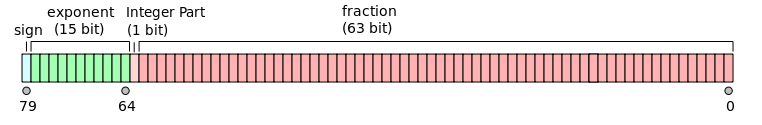
\includegraphics[scale=0.66]{appendix/x86/762px-X86_Extended_Floating_Point_Format.png}
\caption{\IFRU{Формат значения \IT{long double}\protect\footnotemark}
{\IT{long double} value format\protect\footnotemark}}
\end{figure}

\footnotetext{\IFRU{иллюстрация взята из}{illustration taken from} wikipedia}

\label{FPU_control_word}
\subsubsection{\IFRU{Регистр управления}{Control Word}}

\IFRU{Регистр при помощи которого можно задавать поведение}{Register controlling behaviour of the}
\ac{FPU}.

\begin{center}
\begin{tabular}{ | l | l | l | }
\hline
\IFRU{Бит}{Bit} &
\IFRU{Аббревиатура (значение)}{Abbreviation (meaning)} &
\IFRU{Описание}{Description} \\
\hline
0   & IM (Invalid operation Mask) & \\
\hline
1   & DM (Denormalized operand Mask) & \\
\hline
2   & ZM (Zero divide Mask) & \\
\hline
3   & OM (Overflow Mask) & \\
\hline
4   & UM (Underflow Mask) & \\
\hline
5   & PM (Precision Mask) & \\
\hline
7   & IEM (Interrupt Enable Mask) & \IFRU{Разрешение исключений, по умолчанию 1 (запрещено)}
{Exceptions enabling, 1 by default (disabled)} \\
\hline
8, 9 & PC (Precision Control) & \IFRU{Управление точностью}{} \\
     &                        & 00 ~--- 24 \IFRU{бита}{bits} (REAL4) \\
     &                        & 10 ~--- 53 \IFRU{бита}{bits} (REAL8) \\
     &                        & 11 ~--- 64 \IFRU{бита}{bits} (REAL10) \\
\hline
10, 11 & RC (Rounding Control) & \IFRU{Управление округлением}{} \\
       &                       & 00 ~--- \IFRU{(по умолчанию) округлять к ближайшему}{(by default) round to nearest} \\
       &                       & 01 ~--- \IFRU{округлять к}{round toward} $-\infty$ \\
       &                       & 10 ~--- \IFRU{округлять к}{round toward} $+\infty$ \\
       &                       & 11 ~--- \IFRU{округлять к}{round toward} $0$ \\
\hline
12 & IC (Infinity Control) & 0 ~--- (\IFRU{по умолчанию}{by default}) \IFRU{считать}{treat} $+\infty$ \AndENRU $-\infty$ \IFRU{за беззнаковое}{as unsigned} \\
   &                       & 1 ~--- \IFRU{учитывать и}{respect both} $+\infty$ \AndENRU $-\infty$ \\
\hline
\end{tabular}
\end{center}

\IFRU{Флагами}{The} PM, UM, OM, ZM, DM, IM 
\IFRU{задается, генерировать ли исключения в случае соответствующих ошибок}
{flags are defining if to generate exception in case of corresponding errors}.

\subsubsection{\IFRU{Регистр статуса}{Status Word}}

\label{FPU_status_word}
\IFRU{Регистр только для чтения}{Read-only register}.

\begin{center}
\begin{tabular}{ | l | l | l | }
\hline
\IFRU{Бит}{Bit} &
\IFRU{Аббревиатура (значение)}{Abbreviation (meaning)} &
\IFRU{Описание}{Description} \\
\hline
15   & B (Busy) & \IFRU{Работает ли сейчас FPU}{Is FPU do something} (1)
\IFRU{или закончил и результаты готовы}{or results are ready} (0) \\
\hline
14   & C3 & \\
\hline
13, 12, 11 & TOP & \IFRU{указывает, какой сейчас регистр является нулевым}
{points to the currently zeroth register} \\
\hline
10 & C2 & \\
\hline
9  & C1 & \\
\hline
8  & C0 & \\
\hline
7  & IR (Interrupt Request) & \\
\hline
6  & SF (Stack Fault) & \\
\hline
5  & P (Precision) & \\
\hline
4  & U (Underflow) & \\
\hline
3  & O (Overflow) & \\
\hline
2  & Z (Zero) & \\
\hline
1  & D (Denormalized) & \\
\hline
0  & I (Invalid operation) & \\
\hline
\end{tabular}
\end{center}

\IFRU{Биты}{The} SF, P, U, O, Z, D, I \IFRU{сигнализируют об исключениях}
{bits are signalling about exceptions}.

\IFRU{О}{About the} C3, C2, C1, C0 \IFRU{читайте больше}{read more}: (\ref{Czero_etc}).

N.B.: \IFRU{когда используется регистр ST(x), FPU прибавляет $x$ к TOP по модулю 8 и получается номер
внутреннего регистра}{When ST(x) is used, FPU adds $x$ to TOP (by modulo 8) and that is how it gets 
internal register's number}.

\subsubsection{Tag Word}

\IFRU{Этот регистр отражает текущее содержимое регистров чисел}
{The register has current information about number's registers usage}.

\begin{center}
\begin{tabular}{ | l | l | l | }
\hline
\IFRU{Бит}{Bit} & \IFRU{Аббревиатура (значение)}{Abbreviation (meaning)} \\
\hline
15, 14 & Tag(7) \\
\hline
13, 12 & Tag(6) \\
\hline
11, 10 & Tag(5) \\
\hline
9, 8 & Tag(4) \\
\hline
7, 6 & Tag(3) \\
\hline
5, 4 & Tag(2) \\
\hline
3, 2 & Tag(1) \\
\hline
1, 0 & Tag(0) \\
\hline
\end{tabular}
\end{center}

\IFRU{Для каждого тэга}{For each tag}:

\begin{itemize}
\item
00 ~--- \IFRU{Регистр содержит ненулевое значение}{The register contains a non-zero value}
\item
01 ~--- \IFRU{Регистр содержит 0}{The register contains 0}
\item
10 ~--- \IFRU{Регистр содержит специальное число}{The register contains a special value} 
(\ac{NAN}, $\infty$, \OrENRU \IFRU{денормализованное число}{denormal})
\item
11 ~--- \IFRU{Регистр пуст}{The register is empty}
\end{itemize}

\subsection{SIMD-\IFRU{регистры}{registers}}

\subsubsection{MMX-\IFRU{регистры}{registers}}

8 64-\IFRU{битных регистров}{bit registers}: MM0..MM7.

\subsubsection{SSE \AndENRU AVX-\IFRU{регистры}{registers}}

\index{x86-64}
SSE: 8 128-\IFRU{битных регистров}{bit registers}: XMM0..XMM7.
\IFRU{В}{In the} x86-64 \IFRU{добавлено еще 8 регистров}{8 more registers were added}: XMM8..XMM15.

AVX \IFRU{это расширение всех регистры до 256 бит}{is the extension of all these registers to 256 bits}.

\subsection{\RU{Отладочные регистры}\EN{Debugging registers}}

\RU{Применяются для работы с т.н.}\EN{Used for} hardware breakpoints\EN{ control}.

\begin{itemize}
	\item DR0 --- \RU{адрес точки останова}\EN{address of breakpoint} \#1
	\item DR1 --- \RU{адрес точки останова}\EN{address of breakpoint} \#2
	\item DR2 --- \RU{адрес точки останова}\EN{address of breakpoint} \#3
	\item DR3 --- \RU{адрес точки останова}\EN{address of breakpoint} \#4
	\item DR6 --- \RU{здесь отображается причина останова}\EN{a cause of break is reflected here}
	\item DR7 --- \RU{здесь можно задать типы точек останова}\EN{breakpoint types are set here}
\end{itemize}

\subsubsection{DR6}
\myindex{x86!\Registers!DR6}

\begin{center}
\begin{tabular}{ | l | l | }
\hline
\headercolor\ \RU{Бит}\EN{Bit} (\RU{маска}\EN{mask}) &
\headercolor\ \RU{Описание}\EN{Description} \\
\hline
0 (1)       &  B0 --- \RU{сработала точка останова \#1}\EN{breakpoint \#1 has been triggered} \\
\hline
1 (2)       &  B1 --- \RU{сработала точка останова \#2}\EN{breakpoint \#2 has been triggered} \\
\hline
2 (4)       &  B2 --- \RU{сработала точка останова \#3}\EN{breakpoint \#3 has been triggered} \\
\hline
3 (8)       &  B3 --- \RU{сработала точка останова \#4}\EN{breakpoint \#4 has been triggered} \\
\hline
13 (0x2000) &  BD --- \RU{была попытка модифицировать один из регистров DRx.}
               \EN{modification attempt of one of the DRx registers.} \\
            &  \RU{может быть выставлен если бит GD выставлен.}
	       \EN{may be raised if GD is enabled} \\
\hline
14 (0x4000) &  BS --- \RU{точка останова типа single step (флаг TF был выставлен в EFLAGS)}
               \EN{single step breakpoint (TF flag has been set in EFLAGS)}. \\
	    &  \RU{Наивысший приоритет. Другие биты также могут быть выставлены}
	       \EN{Highest priority. Other bits may also be set}. \\
\hline
% TODO: describe BT
15 (0x8000) &  BT (task switch flag) \\
\hline
\end{tabular}
\end{center}

N.B. \RU{Точка останова single step это срабатывающая после каждой инструкции}
\EN{A single step breakpoint is a breakpoint which occurs after each instruction}.
\RU{Может быть включена выставлением флага TF в EFLAGS}
\EN{It can be enabled by setting TF in EFLAGS} (\myref{EFLAGS}).

\subsubsection{DR7}
\myindex{x86!\Registers!DR7}

\RU{В этом регистре задаются типы точек останова}\EN{Breakpoint types are set here}.

\small
\begin{center}
\begin{tabular}{ | l | l | }
\hline
\headercolor\ \RU{Бит}\EN{Bit} (\RU{маска}\EN{mask}) &
\headercolor\ \RU{Описание}\EN{Description} \\
\hline
0 (1)       &  L0 --- \RU{разрешить точку останова}\EN{enable breakpoint} \#1 \RU{для текущей задачи}\EN{for the current task} \\
\hline
1 (2)       &  G0 --- \RU{разрешить точку останова}\EN{enable breakpoint} \#1 \RU{для всех задач}\EN{for all tasks} \\
\hline
2 (4)       &  L1 --- \RU{разрешить точку останова}\EN{enable breakpoint} \#2 \RU{для текущей задачи}\EN{for the current task} \\
\hline
3 (8)       &  G1 --- \RU{разрешить точку останова}\EN{enable breakpoint} \#2 \RU{для всех задач}\EN{for all tasks} \\
\hline
4 (0x10)    &  L2 --- \RU{разрешить точку останова}\EN{enable breakpoint} \#3 \RU{для текущей задачи}\EN{for the current task} \\
\hline
5 (0x20)    &  G2 --- \RU{разрешить точку останова}\EN{enable breakpoint} \#3 \RU{для всех задач}\EN{for all tasks} \\
\hline
6 (0x40)    &  L3 --- \RU{разрешить точку останова}\EN{enable breakpoint} \#4 \RU{для текущей задачи}\EN{for the current task} \\
\hline
7 (0x80)    &  G3 --- \RU{разрешить точку останова}\EN{enable breakpoint} \#4 \RU{для всех задач}\EN{for all tasks} \\
\hline
8 (0x100)   &  LE --- \RU{не поддерживается, начиная с P6}\EN{not supported since P6} \\
\hline
9 (0x200)   &  GE --- \RU{не поддерживается, начиная с P6}\EN{not supported since P6} \\
\hline
13 (0x2000) &  GD --- \RU{исключение будет вызвано если какая-либо инструкция MOV}
			\EN{exception is to be raised if any MOV instruction} \\
            & \RU{попытается модифицировать один из DRx-регистров}
			\EN{tries to modify one of the DRx registers} \\
\hline
16,17 (0x30000)    &  \RU{точка останова}\EN{breakpoint} \#1: R/W --- \RU{тип}\EN{type} \\
\hline
18,19 (0xC0000)    &  \RU{точка останова}\EN{breakpoint} \#1: LEN --- \RU{длина}\EN{length} \\
\hline
20,21 (0x300000)   &  \RU{точка останова}\EN{breakpoint} \#2: R/W --- \RU{тип}\EN{type} \\
\hline
22,23 (0xC00000)   &  \RU{точка останова}\EN{breakpoint} \#2: LEN --- \RU{длина}\EN{length} \\
\hline
24,25 (0x3000000)  &  \RU{точка останова}\EN{breakpoint} \#3: R/W --- \RU{тип}\EN{type} \\
\hline
26,27 (0xC000000)  &  \RU{точка останова}\EN{breakpoint} \#3: LEN --- \RU{длина}\EN{length} \\
\hline
28,29 (0x30000000) &  \RU{точка останова}\EN{breakpoint} \#4: R/W --- \RU{тип}\EN{type} \\
\hline
30,31 (0xC0000000) &  \RU{точка останова}\EN{breakpoint} \#4: LEN --- \RU{длина}\EN{length} \\
\hline
\end{tabular}
\end{center}
\normalsize

\RU{Так задается тип точки останова}\EN{The breakpoint type is to be set as follows} (R/W):

\begin{itemize}
\item 00 --- \RU{исполнение инструкции}\EN{instruction execution}
\item 01 --- \RU{запись в память}\EN{data writes}
\item 10 --- \RU{обращения к I/O-портам (недоступно из user-mode)}\EN{I/O reads or writes (not available in user-mode)}
\item 11 --- \RU{обращение к памяти (чтение или запись)}\EN{on data reads or writes}
\end{itemize}

N.B.: \RU{отдельного типа для чтения из памяти действительно нет}
\EN{breakpoint type for data reads is absent, indeed}. \\
\\
\RU{Так задается длина точки останова}\EN{Breakpoint length is to be set as follows} (LEN):

\begin{itemize}
\item 00 --- \RU{1 байт}\EN{one-byte}
\item 01 --- \RU{2 байта}\EN{two-byte}
\item 10 --- \RU{не определено для 32-битного режима, 8 байт для 64-битного}
		\EN{undefined for 32-bit mode, eight-byte in 64-bit mode}
\item 11 --- \RU{4 байта}\EN{four-byte}
\end{itemize}


% TODO: control registers
